\chapter{Testing Environment}
\label{chap:testing_environment}
	
	\par In this chapter is described the whole environment where I settled the investigation of each Android mobile application discussed in this thesis.
	\par Core of the environment is the \textit{Android Studio} framework, offering both an Integrated Development Environment (IDE) and testing features for Android mobile applications. Here I configured an emulated device where I could run the application cases I investigated.
	\par Once installed the specific application I had to analyze the \textit{network traffic} generated by itself. Generally it is rare a single tool is perfect for all the applications to analyze, this is the reason why I used different tools to inspect the network traffic generated by an application, instead of just sticking with one tool. Starting from the standard-de-facto in packet inspection \textit{Wireshark} program, ending to tools acting like proxy servers between the client application and the server. Some of these tools are able to automatically install and configure a man (MitM attack [\ref{subsec:mitm}]) in the middle of the communication, others might need some manually configuration. \newline
	The whole amount of informations exchanged between application and server is hidden somewhere in the communication. It might be more or less difficult to find them, but all the informations are there, in those packets.
	\par Some tools revealed to be really useful while investigating the network traffic of the applications. Dynamic instrumentations tools are softwares able to inspect at runtime what is happening in the mobile application. On the other way, static instrumentation tools offer a view of the application basing on its code.
	
	\section{Android Studio}
		\par \textbf{Android Studio} is the center of the testing environment. Other than a complex IDE software, it provides a complete testing suite for Android mobile applications. Once installed the software, it enables the access to the Android Device Manager tool, where the user can create an emulator for a specific Android device choosing among phones, tablets, wearOS or TVs. 
		In this section I will explain how I prepared the android virtual device in order to obtain a working environment that made possible the application investigation.
		
		\subsection{Android Virtual Device (AVD)}
			For my purpose study case I created an \textit{Android Virtual Device} (AVD) phone with the same properties of the \textit{Pixel 3a} phone developed by Google, that is \textit{5.6''} screen size, \textit{1080x2220} resolution, \textit{440dpi} density. The device is running \textit{Android 13}, also known as \textit{Tiramisu} version, or \textit{API 33}, on \textit{x86\_64} architecture. In the really first step while selecting the hardware we would like to use for the virtual device, some device definitions are enabled to run the Play Store software, and so it is for our Pixel 3a device. This is really useful since I had not to download and install manually each applications on the device. Indeed it is made possible using the Google Play store directly from the emulated device. 
			\par Once created the new virtual device (in my case called \textit{''Pixel\_3a\_API\_33\_-\_Data\_Leak\_Detection''}), it is possible to run it through the Android Device Manager. For simplicity I created a simple \textit{.bat} file to run the virtual device without the need to open Android Studio everytime. Indeed there is a file called \textit{emulator.exe} in a the folder where we installed the Android SDK. We can simply open the emulator by command line passing the name of our AVD and some optional arguments. Here it is how my command looks like:
\begin{lstlisting}[language=bash, caption={run\_AVD.bat}]
C:\<Android_folder>\Sdk\emulator\emulator -feature -Vulkan -memory 2048 -netdelay none -netspeed full -avd Pixel_3a_API_33_-_Data_Leak_Detection
\end{lstlisting}
		\par More specifically the \textit{-feature -Vulkan} argument will force the emulator to do not use the \textit{Vulkan} graphic library. Since Android API 30 lots of android applications, such as Google Chrome, use this library to boost its performance. Anyway in some devices, especially for the emulated ones, might result in a massive slow rendering time. Other arguments are specifying to dedicate 2 Gb of RAM memory for the device, to not impose limits on the network speed and to not simulate any network delay.
			\par Here there is the full property list of the device I used:
			\begin{center}
				\begin{tabular}{ |p{5cm}||p{9cm}| }
					 \hline
					 \multicolumn{2}{|c|}{Android Virtual Device (AVD) Properties} \\
					 \hline
					 \hline
					 avd.ini.displayname & Pixel 3a API 33 - Data Leak Detection \\
					 AvdId & Pixel\_3a\_API\_33\_-\_Data\_Leak\_Detection \\
					 image.androidVersion.api & 33 \\
					 image.sysdir.1 & system-images/android-33/google\_apis\_playstore/x86\_64/ \\
					 tag.id & google\_apis\_playstore \\
					 hw.device.name & pixel\_3a \\
					 hw.device.manufacturer & Google \\
					 hw.cpu.ncore & 4 \\
					 hw.ramSize & 1536 \\
					 vm.heapSize & 228 \\
					 hw.lcd.width & 1080 \\
					 hw.lcd.height & 2220 \\
					 hw.gpu.enabled & yes \\
					 hw.gps & yes \\					 
					 hw.accelerometer & yes \\
					 runtime.network.speed & full\\
					 runtime.network.latency & none \\
					 \hline
				\end{tabular}
			\end{center}

			%\begin{figure}[!ht]    
				%\centering   
				%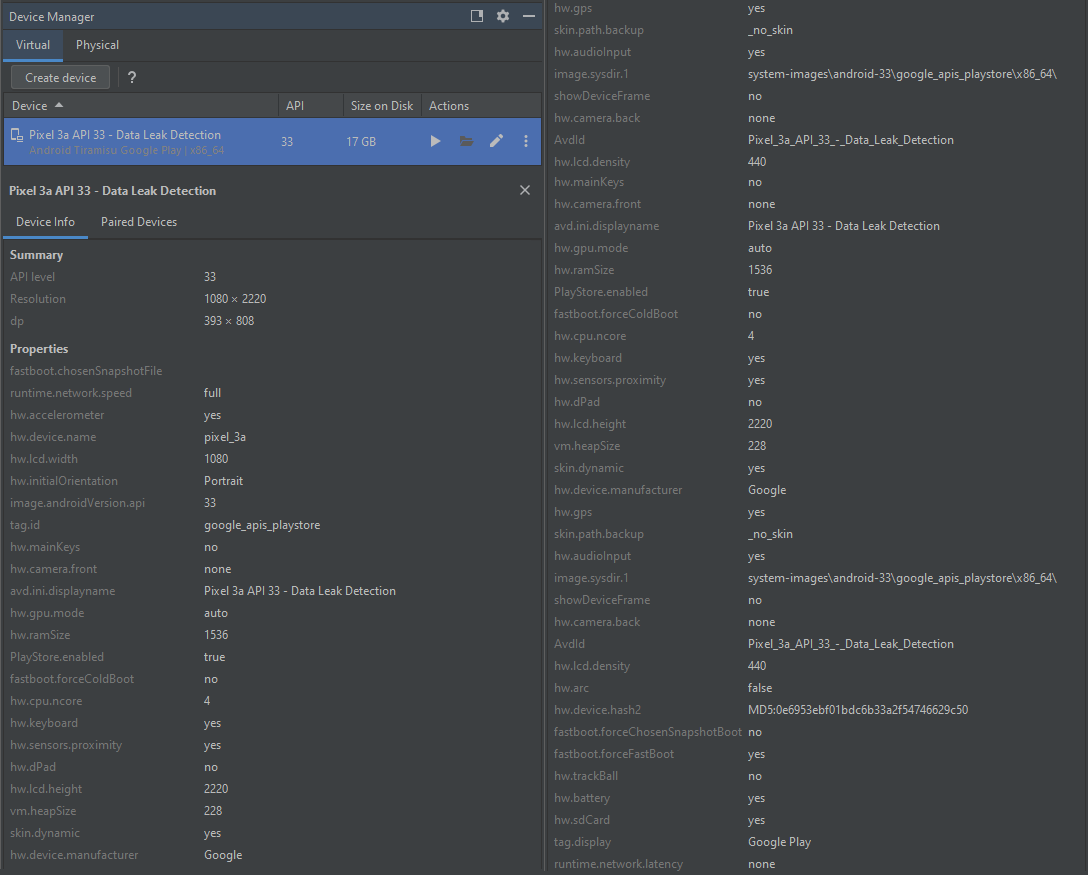
\includegraphics[width=0.9\textwidth]{./images/avd_splitted.png}
			    	%\caption{Android Virtual Device (AVD) specifics}
			%\end{figure}
			
		\subsection{Root privileges on virtual device}
			\par After having succesfully created the AVD, it can result useful to get the \textit{root privileges} on the device. In our case it is really mandatory since what we are going to do is intercept the communication protocol in the middle between application and server. As explained in the Section \ref{subsec:mitm}, the client application needs to trust the proxy server, and this is done by checking its certificate. Starting from the release of version \textit{Nougat} (API $\ge$ 24), of Android operative system, it changed the behaviour adopted by android applications in trusting users. If before the application was checking both \textit{user certificates} and \textit{system certificates}, now it will check exclusively the installed system level certificates, therefore root privileges are mandatory. \newline
			\par There are so many tools that let a user obtain the root privileges on his phone. I personally have used the \textit{rootAVD} tool available online \cite{rootAVD}. The procedure is really simple, firstly run the command with argument \textit{ListAllAVDs} to list all the AVDs on the machine. We will obtain the full path of our AVDs, that we will pass as argument when executing the tool from command line. The tool will make use the \textit{adb} tool that Android Studio brings together with its development tools, so it is worth it to explain what it is.
		
		\subsection{Android Debug Bridge (adb)}
			\par As I said Android Studio offers a complete set of features to run and test android application. In particular by installing the \textit{Android SDK Platform Tools} package from Android Studio, we will obtain a set of tools that make possible the debug of our application. \newline
			One of the most important tools is the Android Debug Bridge, more noticed as \textit{adb}. It is a command line tool that let the user directly communicate with an Android device, let it be a physical or emulated device. Basically it is a client-server program that runs both on our machine and Android device. There is then a client, that is the command line tool, a daemon \textit{adbd} running in the background of the Android device, and a server managing the connection between client and daemon. For a complete understanding of the adb tool check the Android Developer guide \cite{adb}.
		
	\section{Network traffic analysis}
		\par Once the virtual device is well configured as described above, let's start introducing some network tool I used for my study cases. Each one of them has some strengths, one tool might works for an application but not work for another. They are listed below in order of complexity. \textit{HttpToolkit} and \textit{BurpSuite} are network traffic interceptors, that means every connection outgoing from our device will be intercepted by these applications, letting the user to inspect more or less accurately how the request were formed. \textit{Wireshark} on the other way is a packet sniffing tool, meaning that it will capture any packet in the network, regardless of the protocol or the port used. 
		
		\subsection{HttpToolkit}
		\label{sec:http_toolkit}
			\par HttpToolkit\cite{http_toolkit} is an open-source tool for debugging, testing and building with HTTP(S). The strength of this tool relies on its simplicity for configuring the environment. Once downloaded the application it requires to be connected to a source of traffic. HttpToolkit provides a variety of available sources, from the most famous browser (Chrome, Firefox, Safari, Edge), up to more complicated environment, such as Docker containers, virtual machines, Android devices or iOS devices. In this case the network source to monitor is the Android virtual device where the applications will run. The program itself will notify the user which are the available sources of traffic at the start up. Since the scope of the study is investigating applications running on the android emulator, it is needed to download from Google Play the HttpToolkit application also on the virtual device. Once installed the android app, the HttpToolkit running on the computer will automatically notice the new source called \textit{''Android device via ADB''}. Just click on it and the whole proxy system is automatically configured. \newline
			\par In this phase it is crucial to understand what is happening:
			\begin{itemize}
				\item HttpToolkit will inject a custom certificate on our device, communicating with it through ADB. Since we also have the root privileges on the android emulator, the certificate willl be placed in the folder of the \textit{System Certificates} that is \textit{/system/etc/security/cacerts} in the Android device. \newline
				\item The respective HttpToolkit Android application will be activated in order to set up a VPN, redirecting the whole network traffic directly via the Android Debug Bridge to the main HttpToolkit program running on the computer. \newline
				\item HttpToolkit will copy to the device, again via ADB, a file containing the command used to start up the Android Google Chrome application. 
\begin{lstlisting}
chrome --ignore-certificate-errors-spki-list=<hash_digest>
\end{lstlisting}
This specific command will bypass the Certification Transparency check described in the section \ref{subsec:certification_transparency}. The command looks like the following, where \textit{hash\_digest} is the hash digest of the SSL certificate used by the tool.\newline
			\end{itemize} 
			
			\par All these steps are done automatically from the program itself. Indeed this tool requires almost no configuration on the user side, aside from the preparation of the AVD discussed in the above section.
			\par	As described in the certificate verification [Section \ref{subsec:certificate_verification}] and MiTM [Section \ref{subsec:mitm}], this is the moment in which the HTTP(S) requests outgoing from the application case are intercepted by HttpToolkit, showing precisely each request detail. Then they are forwarded to the application server. Same happens for the HTTP(S) responses. Moreover in case certificate is rejected by the application, that means some certificate pinning procedure has been adopted, the tool will notify us.
			\par Anyway HttpToolkit is only able to intercept the HTTP(S) protocol, that is enough for most of the Android applications. In case the application will communicate in a different protocol (QUIC for example) the requests are not visible to this tool, so we will need a different network tool.
		
		\subsection{BurpSuite}
		\label{sec:burp_suite}
			\par \textbf{Burp Suite} is one of the most famous web security suite. It is available in different versions: \textit{Community Edition}, \textit{Professional Edition} and \textit{Enterprise Edition}. The first one is more than enough for personal and research purposes and it is the one I used. It contains the essential toolkit letting the user to be able to set up a proxy and perform a MiTM interception while analyzing the content of the requests passing through the proxy. Differently from HttpToolkit it is more flexible in terms of protocols able to intercept, for example HTTP/3 over QUIC, and it is way more customizable. Indeed it let the user set up specific listeners (address and port), or import/export specific CA certificates with which decode the encrypted messages. Moreover it provide a specific \textit{''Repeater''} tab where the user can manually craft or modify already existing requests and forward them to the endpoint. This last one feature is a routine very useful that I used for every application case.
			\par On the other side, this tool is not auto-configured to intercept traffic coming from mobile device. Everything has to be manually set on both proxy side and mobile device side. Theoretically the configuration steps to enable the interception of HTTPS requests are the same described in the previous section, that HttpToolkit was doing automatically, but instead in this case have to be applied manually \cite{burp_suite}:
			\begin{itemize}
				\item From the Proxy options, export the CA certificate in \textit{DER format}. This is the certificate that we will manually have to install as system-level in the Android operative system. Anyway Android will read only a \textit{PEM format} certificate. Once exported the certificate we will need to convert the certificate using the \textit{openssl} tool available for every platform. But this is not enough, in fact the certificate needs to have the filename equal to the \textit{subject\_hash\_old} value (that is the \textit{hash} of the certificate subject name computed by OpenSSL with the \textit{''old''} version 1.0) appended with \textit{0}. The command lines to achieve the result are:
\begin{lstlisting}
$ openssl x509 -inform DER -in <cacert>.der -out <cacert>.pem
$ openssl x509 -inform PEM -subject_hash_old -in <cacert>.pem | head -1
$ mv cacert.pem <hash_digest>.0
\end{lstlisting}
				This certificate has to be pushed to the device, and then moved to the \textit{/system/etc/security/cacerts/} folder, modifying its permissions. Notice that the ADB tool cannot execute commands as root user while using \textit{play\_store} images of Android (kernel images builtin with Google Play application) as in our case. Firstly it has to be pushed on the \textit{/sdcard/} location and than moved with the \textit{adb shell -c ''mv <source> <dest>''}:
\begin{lstlisting}
$ adb push <hash_digest>.0 /sdcard/
$ adb shell su -c ''mv /sdcard/<hash_digest>.0 /system/etc/security/cacerts/''
$ adb shell su -c ''chmod 644 /system/etc/security/cacerts/<hash_digest>.0''
\end{lstlisting}
				Be aware that rebooting the device will remove the certificate and the procedure has to be done again.\newline
				\item From Proxy options, we have to set up the correct listener. In our case we manually insert the specific IP address of our machine (since the traffic generated from the emulator will have that IP address) or just we can select \textit{All interfaces}. The port can be anyone available, let it be \textit{8082}. Respectively on the Android emulator we have to redirect the outgoing traffic to that proxy. A common proxy setting in the WiFi connection is fine: the IP address will be the one of the computer running Burp Suite, the port will be \textit{8082}.\newline
				\item Lastly we will have to fix the Chrome behaviour on the application in order to do not apply Certificate Transparency for that specific certificate. In any case this step is optional since we will not be using Chrome, but the Android application itself.\newline
			\end{itemize} 
			\par After having configured Burp Suite in this way, by clicking on the \textit{Intercept is off} in the \textit{Proxy} tab, we will be able to intercept any request outgoing from the Android emulated device. As well we can consult the HTTP history of the requests. More than this, we can click \textit{Send to Repeater} from a specific request to manually edit the fields, like Headers or Body, and forward it to the endpoint.
		
		\subsection{Wireshark}
		\label{sec:wireshark}
			\par \textbf{Wireshark} is the most famous packet sniffer tool. Differently from the two tools described before, Wireshark is a low level network protocol analyzer meaning that every packet outgoing from the selected Network Card Interface will be captured being able to analyze them. This tool will not differentiate between protocols, every packet will be captured. \newline
			\par Wireshark is a really powerful tool, also able to decrypt TLS communications if provided with the so called \textit{pre-master secret key}. This step is easily possible on Windows, Mac, or Linux operative system by setting an environment variable, so that the browser is enabled to export the secret key used in their encrypted communication. Once exported the pre-master shared keys, it is possible to instruct Wireshark to decode the TLS traffic by using those secret keys. Anyway this is not possible in Android operative system, or at least in this way. In fact it is possible to extract pre-master secret key used by a specific application with Frida (see Section \ref{subsec:frida_sslkeylog}).\newline
			\par Another possible approach in order inspect decrypted TLS communication in Wireshark is by using some other proxy tool capturing the network traffic at proxy level and capable of exporting the packet logs in \textit{.pcap} or \textit{.pcapng} format. Then is possible to open those logs with Wireshark and analyze every packet captured by the proxy.
			\par In this study Wireshark has been used complementarily to the previous tools HttpToolkit and BurpSuite. In particular since it captures any type of communication protocol, I wanted to be sure that the Android application was not communicating with some other protocol different from HTTP(S) or QUIC, and in that case analyze the data exchanged.
	
	\section{Dynamic instrumentation}
		\subsection{Frida}
			
			\subsubsection{SSL Keylog}
			\label{subsec:frida_sslkeylog}
		
		\subsection{Objection}
		
	\section{Static instrumentation}
		\subsection{GDA}
